%\documentclass[prd, nofootinbib, floatfix, 12pt]{revtex4}
%\documentclass[useAMS,usenatbib,11pt,preprint]{aastex}
\documentclass[]{article}

\usepackage[paperwidth=8.5in,paperheight=11in,centering,hmargin=1in,vmargin=1in]{geometry}
\usepackage{amsmath}
\usepackage{amsbsy}

\topmargin0.0cm
\textheight8.5in

\input epsf
\usepackage{amsmath,amssymb,subfigure}
\usepackage{graphicx}
\usepackage{epsfig}
\usepackage{color}
%\usepackage{ulem}
%\usepackage{epstopdf}

\renewcommand{\topfraction}{0.95}
\renewcommand{\bottomfraction}{0.95}





%%%%%%%%%%%%%%%%%%%%%%%%%%%%%%%%%%%%%%%%%%%%%%%%%%%%%%%%%%%%
%%%%%%%%%%%%%%%%%%%%%%%%%%%%%%%%%%%%%%%%%%%%%%%%%%%%%%%%%%%%
%%%%%%%%%%%%%%%%%%%%%%%%%%%%%%%%%%%%%%%%%%%%%%%%%%%%%%%%%%%%

\begin{document} 
\sloppy
\title
{Validation of the Simulations Catalogs}

%\pagerange{\pageref{firstpage}--\pageref{lastpage}}

\label{firstpage}

% \date{\today}

\maketitle 
\section{Introduction \label{sec:intro}}
The purpose of this document is to work in concert with the "Requirements for the 
LSST Simulation Framework" (hereafter Requirements; \cite{requirements}) to validate the
base catalogs and catalogs generation framework for use in the context of
LSST investigations. 
\section{Validation of the Requirements on the Catalog Simulations}
This section will show in detail whether each requirement is being met and if it is not
being met what the impact on the project measureables and design goals is.
\subsection{Requirement 1: The LSST catalogs simulations shall contain representations of stars,
galaxies, asteroids, and variable sources}
\subsubsection{Stars}
Stars are represented as point sources.  SEDs and kenimatics are assigned to stars using SDSS colors produced by the Galfast (\cite{galfast})
model.  A three dimensional dust model is applied to un-extincted magnitudes using the smooth model of \cite{amores} and normalizing to the
measured extinction values from \cite{sfd}.  Binary stars are included in the luminosity funcitons from which the stellar colors are sampled,
but are assumed to be unresoved and non-variable (except for a selection of eclipsing binarys described later).

Stellar  populations in the model:
\begin{itemize}
\item Main Sequence: F,G,K,M,L,T
\item White Dwarf: H and He
\item Red Giant Branch
\item Blue Horizontal Branch
\item RRly
\item Cepheids {\bf XXX check that this is full sky}
\end{itemize}

\subsubsection{Galaxies}
The galaxy model is based on haloes form the Millenium simulation (\cite{millenium}) with physical attributes assigend by \cite{dilucia}.  
Numbers were adjusted to meet observed relations (see \ref{sec:galaxycounts}).  Each galaxy is described by a three component model consisting 
of two Sersic models (bulge and disk) and point source (AGN).  The three are scaled given flux ratios provided by the semi-analytic catalog.  Inclination dependent
dust is applied to the disk.  The bulge can also have internal extinction, but is chosen randomly from a realistic distribution.  The
AGN component is the \cite{vandenberk} mean AGN spectrum.

\subsubsection{Asteroids}
The solar system model is a realization of the \cite{grav} model.  All major groups are represented including: main belts, near earth objects, 
trojans of the major plantes, trans-neptunian objects, and comets.  Each is assigned a carbonaceous or stony composition spectrum.

\subsubsection{Variable sources}
The framework is able to support several types of variability: periodic, stochastic, repeating.  The variability models can be parametric or interpolated.  
To date only mono-chromatic variability has been exercised, but there are no limitations that preclude fully consistent pan-chromatic variability.

Variability models:
\begin{itemize}
\item M-dwarf flares -- full sky
\item AGN/QSOs -- full sky
\item Cepheids -- full sky {\bf XXX check this}
\item RRly -- full sky
\item Eclipsing binaries -- exemplar individuals
\item Am CVn -- exemplar individuals
\item Micro lensing -- exemplar individuals
\end{itemize}

\subsubsection{Algorithmic and Systems Level Analysis Enabled}
The above model of the Universe exercises all the important aspects of the algorithms and systems level concerns currently under investigation
by the project.

Investigations supported:
\begin{itemize}
\item astrometry
\item photometry
\item multi-fit
\item calibration
\item moving objects detection
\item alert production
\item image differencing
\item star galaxy separation
\item coaddition
\end{itemize}

\subsection{Requirement 2: At high Galactic latitudes the average source densities of stars and galaxies
shall be within 18\% of the observed counts (to the 5$\sigma$ point source coadded depth of LSST)}

\subsubsection{Stars}
{\bf XXX I need to do this for the 180. fields and for the Besancon with our dust model.  Also need to add the lat=0 fields if we are going to do them.}
We take six representative fields at varying galactic latitude at two longitudinal values (one toward the bulge and one away).  We compare number 
counts of main sequence stars to the coadded limiting magnitude in i-band {\bf XXX is this to maximize the number of stars detected in the disk?}
 from the galfast model using the composite dust model
of \cite{amores} normalized to \cite{sfd} to the Besancon {\bf sp and reference} model with their dust model.  Figure \ref{fig:scounts_0} shows 
the cumulative number counts as a function of magnitude for the Besancon (dashed) and Galfast (solid) models.  We are interested in the
fractional cumulative contribution.  In Figure \ref{fig:sratio_0} we plot the ratio of Besancon counts to Galfast counts for the six test fields
The dashed lines are the $\pm30\%$ limits for the low latitude sizing model constraints and the dash-dot lines are the $\pm18\%$ limits motivated
by science requirements.  Since the number counts are dominated by the faint end, it's most important where the lines end up at faint magnitudes for 
sizing considerations.  For science consideratons, the single epoch depth is also an interesting location to test the ratios.  For all cases the 
requirements are met at the single epoch depth.  At the coadd depth, all the fields pass the requirements except for the -10 case which under
predicts relative to the Besancon model by ~5\% over the required value.
\begin{figure}
\centering
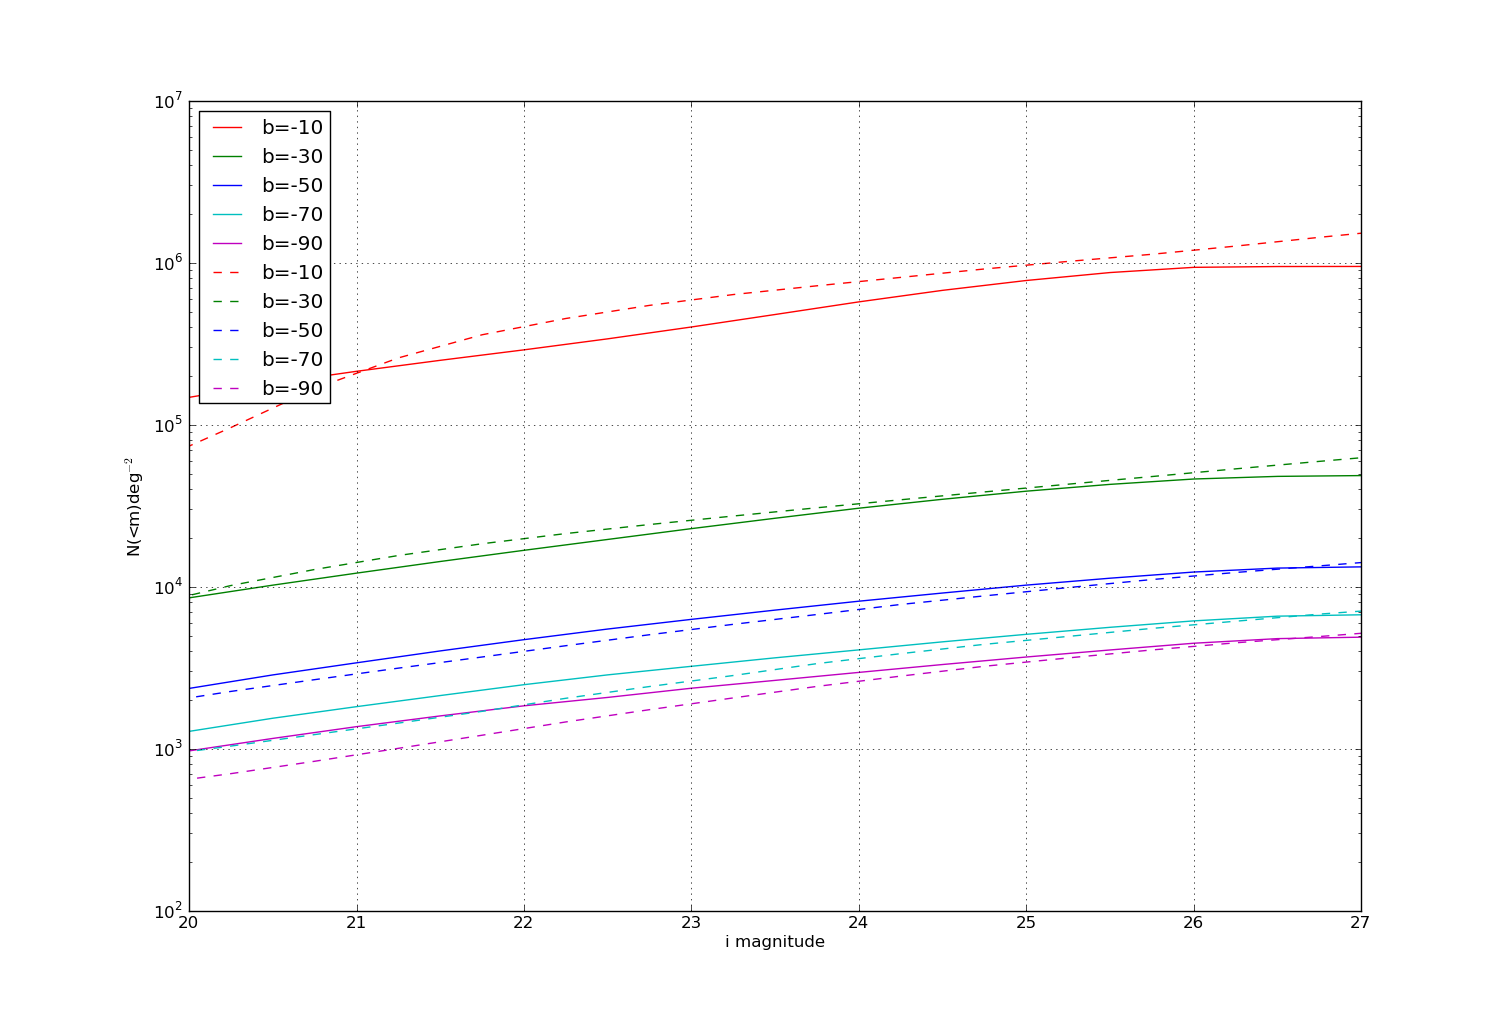
\includegraphics[width=5in]{validation_figures/cumulative_stars.eps}
\caption{Cumulative counts of stars from the Besancon (dashed) and Galfast (solid) models for 5 representative fields toward the galactic bulge \label{fig:scounts_0}}
\end{figure}
\begin{figure}
\centering
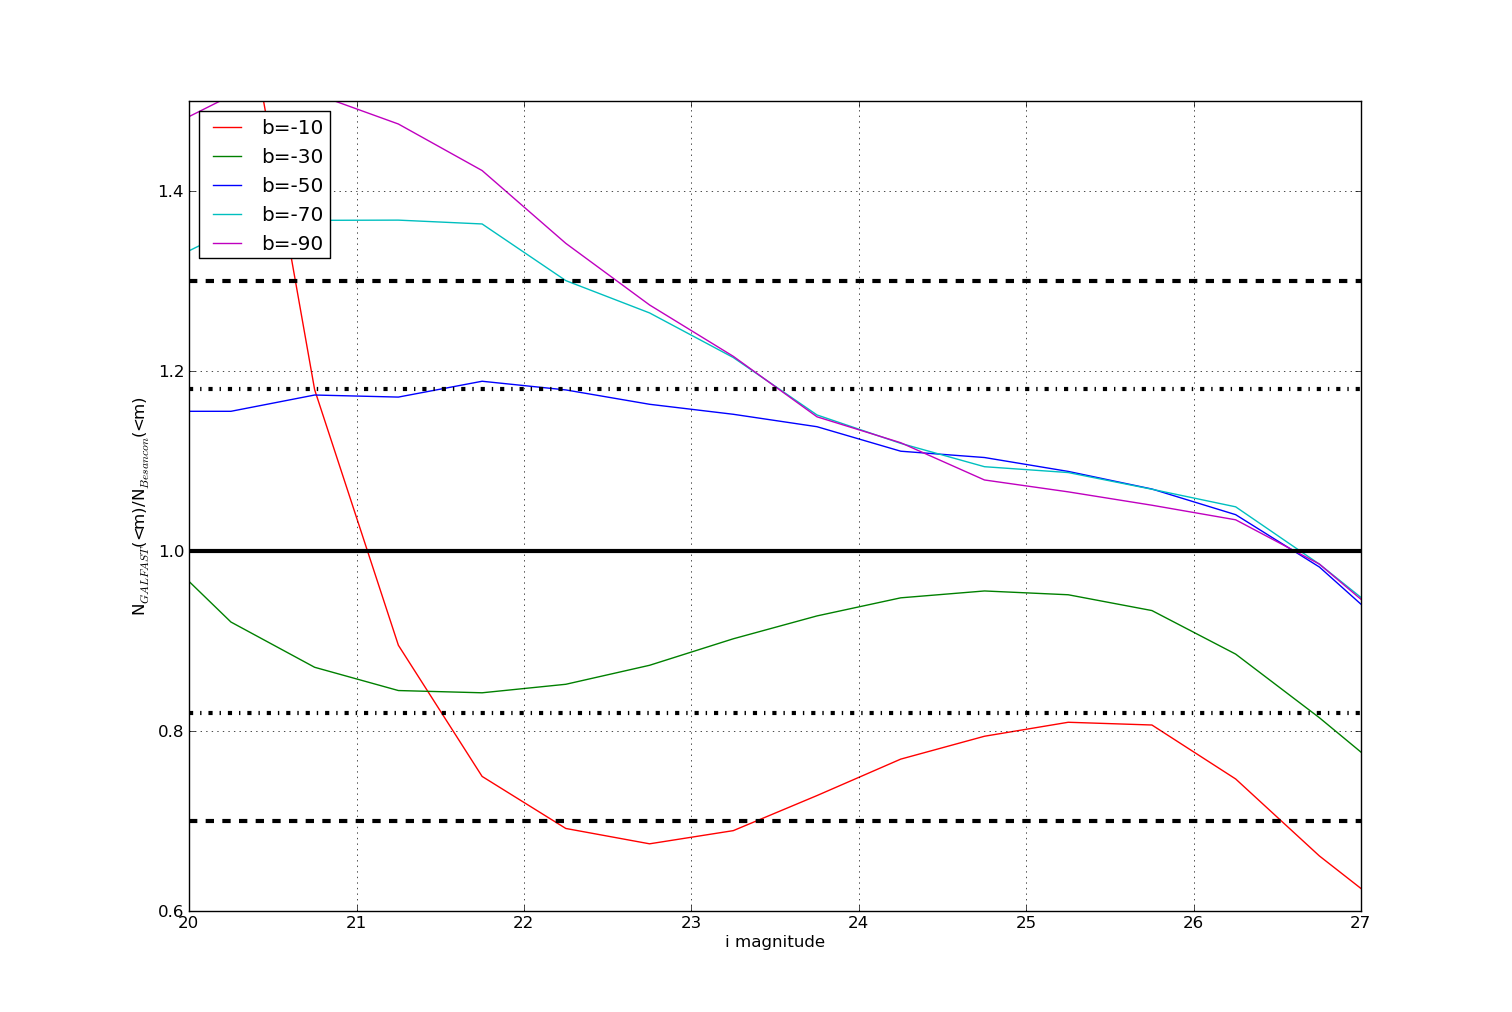
\includegraphics[width=5in]{validation_figures/cumulative_ratio_stars.eps}
\caption{Cumulative ratio of counts of stars from the Besancon and Galfast models for 5 representative fields toward the galactic bulge \label{fig:sratio_0}}
\end{figure}

\subsubsection{Galaxies \label{sec:galcounts}}
We compare the galaxy counts to those provided by the Durham group.  We have taken their compilations from:
{\tt http://star-www.dur.ac.uk/~nm/pubhtml/counts/idata.txt} access on 06/01/2013.  We use only data points with error bars in our analysis.  Using these counts
we noticed that the numbers of galaxies were under predicting at faint magnitudes.  We used a cloning algorithm to push up the number counts at faint magnitudes
while maintianing realistic number counts as a function of redshift.

The result of the nubmer counts as a function of magnitude after the cloning are shown in \ref{fig:gcounts}.  We have chosen the I-band data for comparison to 
minimize the effects of dust extinction which are somewhat uncertain in the Durham compilations.  A single transform of I$_{kc}$ = i$_{AB}$ - 0.5 was applied to
all compliation data.  For comparison with requirements on the sizing model stated in the requirements document, we also plot the cumulative ratio of the best fit polynomial
to the Durham data to the counts from the base catalog.  The goal is $\pm30\%$ to the coadded i-band depth of 26.8.  We see that the base catalog
underpredicts at the faintest magnitudes, but meets the requirement (Figure \ref{fig:gratio}).

\begin{figure}
\centering
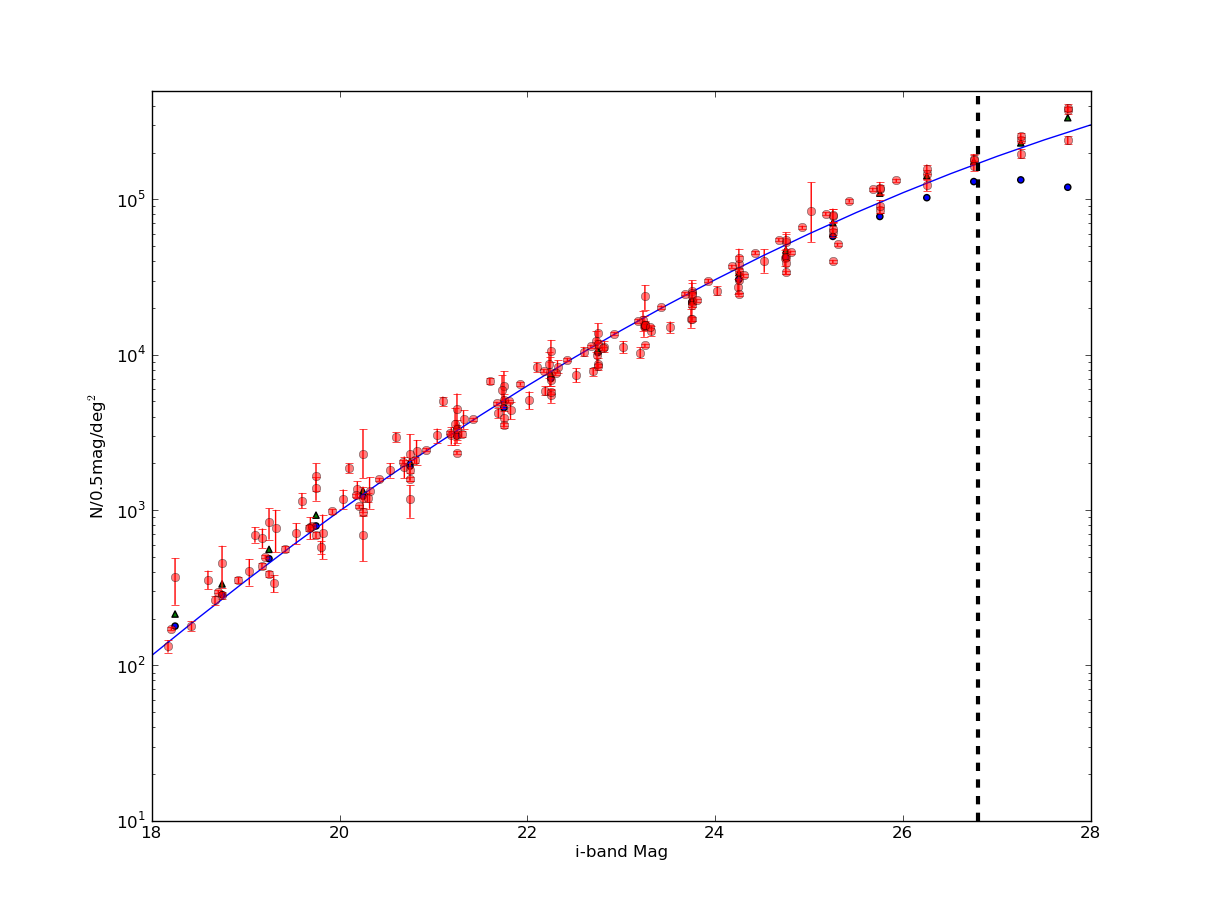
\includegraphics[width=5in]{validation_figures/Ngals-i.eps}
\caption{Durham counts (symbols) compared to the counts from the base catalog \label{fig:gcounts}}
\end{figure}
\begin{figure}
\centering
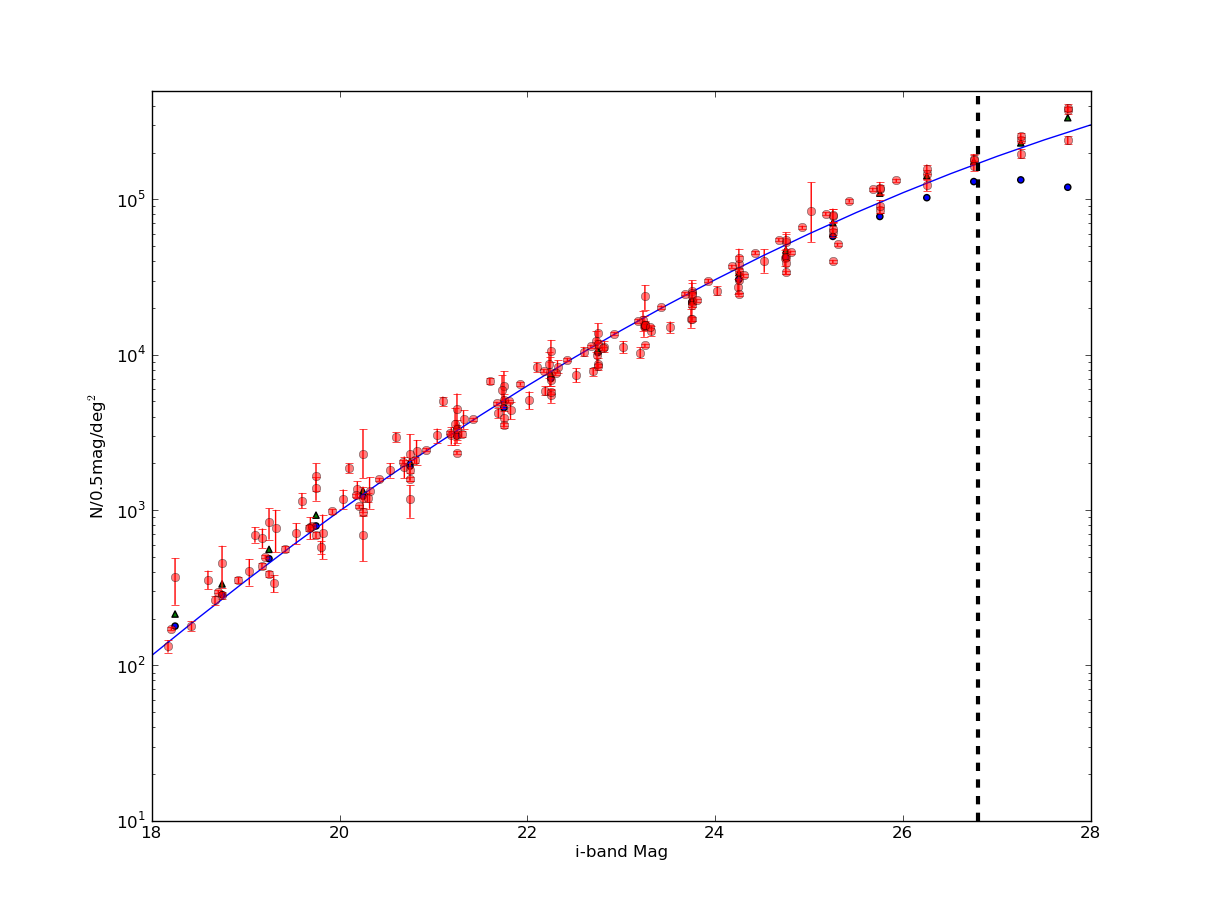
\includegraphics[width=5in]{validation_figures/Ngals-i.eps}
\caption{Durham counts divided by the counts from the base catalog.  Error bars are from adding the error bars from the data points in quadrature. \label{fig:gratio}}
\end{figure}

\subsection{Requirement 3: Size, ellipticity and redshift distributions of galaxies shall be representative of those observed by extant
telescopes and, for a fiducial image quality of 0.7 arcsec, deviations from the observed distributions shall
contribute $< 20\%$ of the observed effective density of galaxies, $n_{eff}$, used in the weak lensing samples (with a fiducial value of
$n_{eff} = 34$ galaxies per arcmin$^2$}
{\bf XXX I still don't don't know exactly these all fit together, so I'm not going to write much until we talk more.}
{\bf XXX I need to to figure out the size comparison.  I may just do what Rob did in the past and compare to HST.}
%\begin{figure}
%\centering
%\includegraphics[width=5in]{validation_figures/COSMO_base_ellip.eps}
s%\caption{\label{fig:ellip}}
%\end{figure}
\begin{figure}
\centering
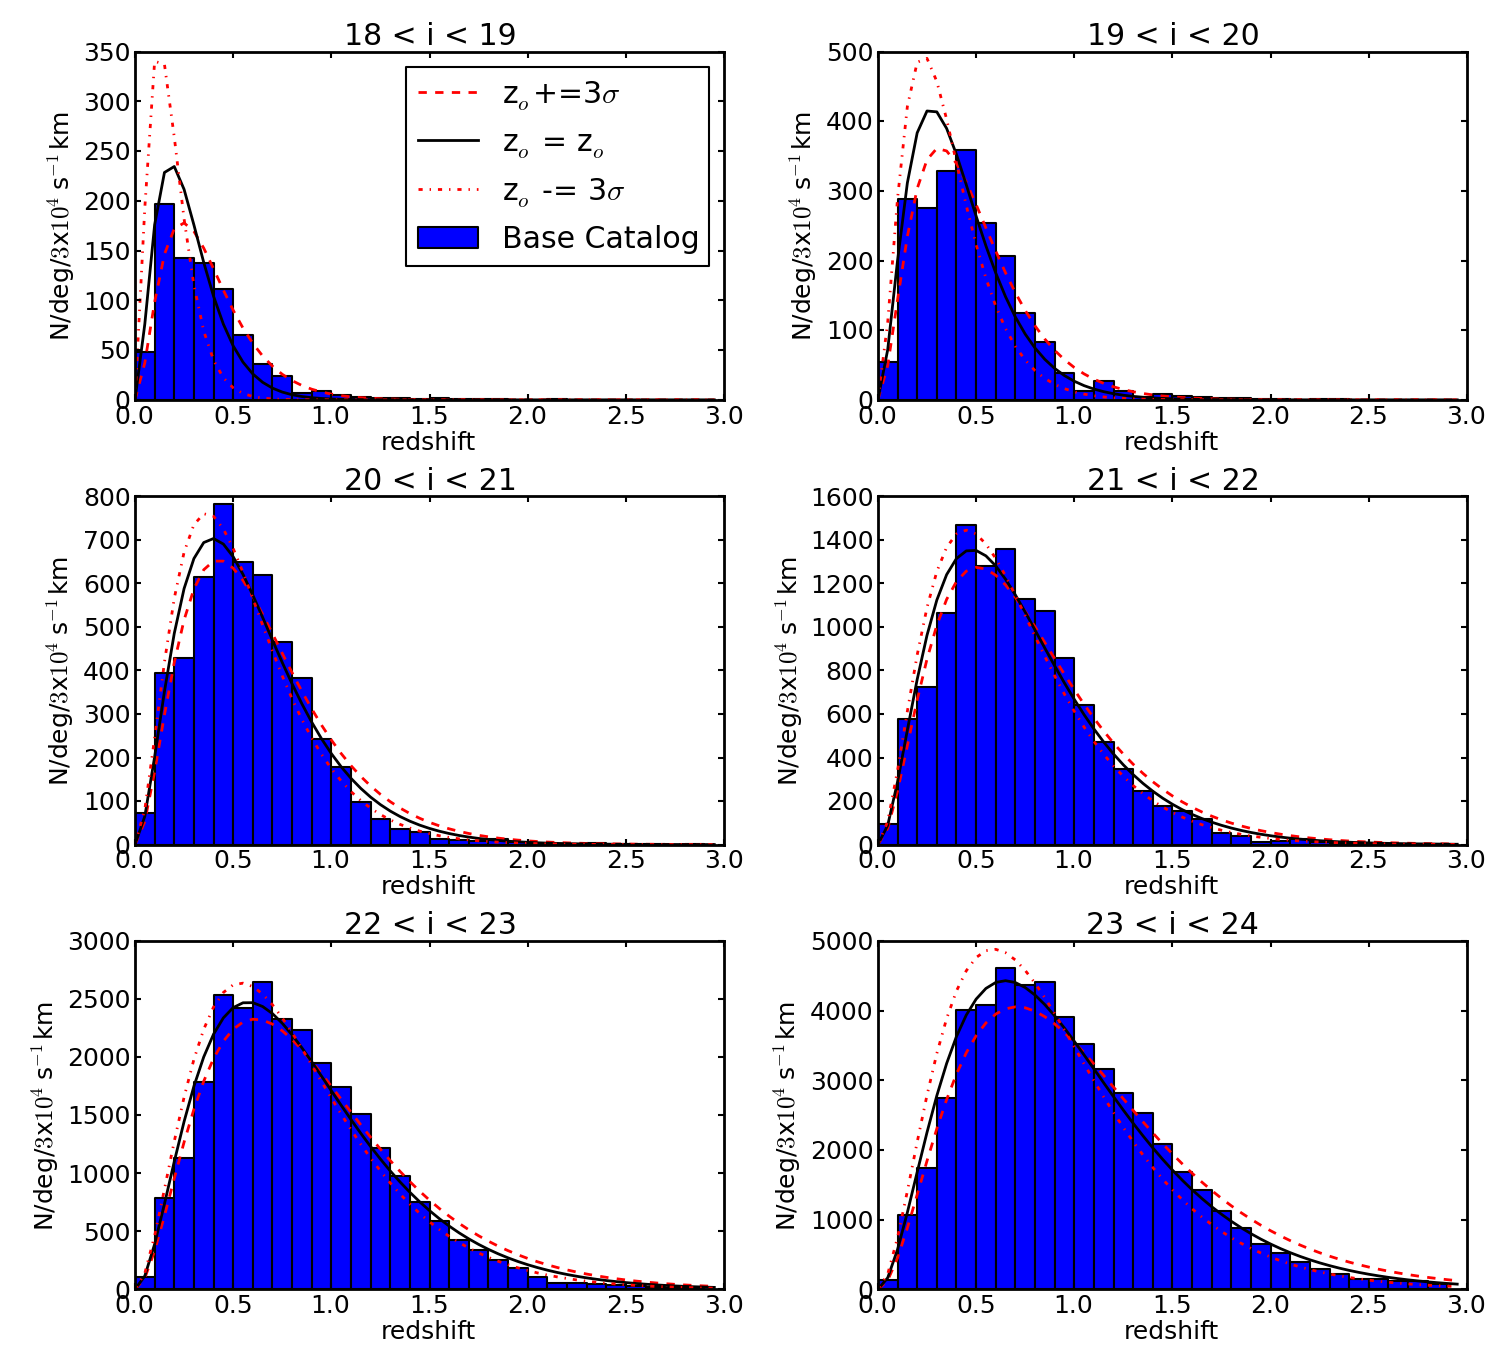
\includegraphics[width=5in]{validation_figures/Nofz_18_24.eps}
\caption{N(z) for 18 to 24 with distribution from \cite{coil}\label{fig:nofz18_24}}
\end{figure}
\begin{figure}
\centering
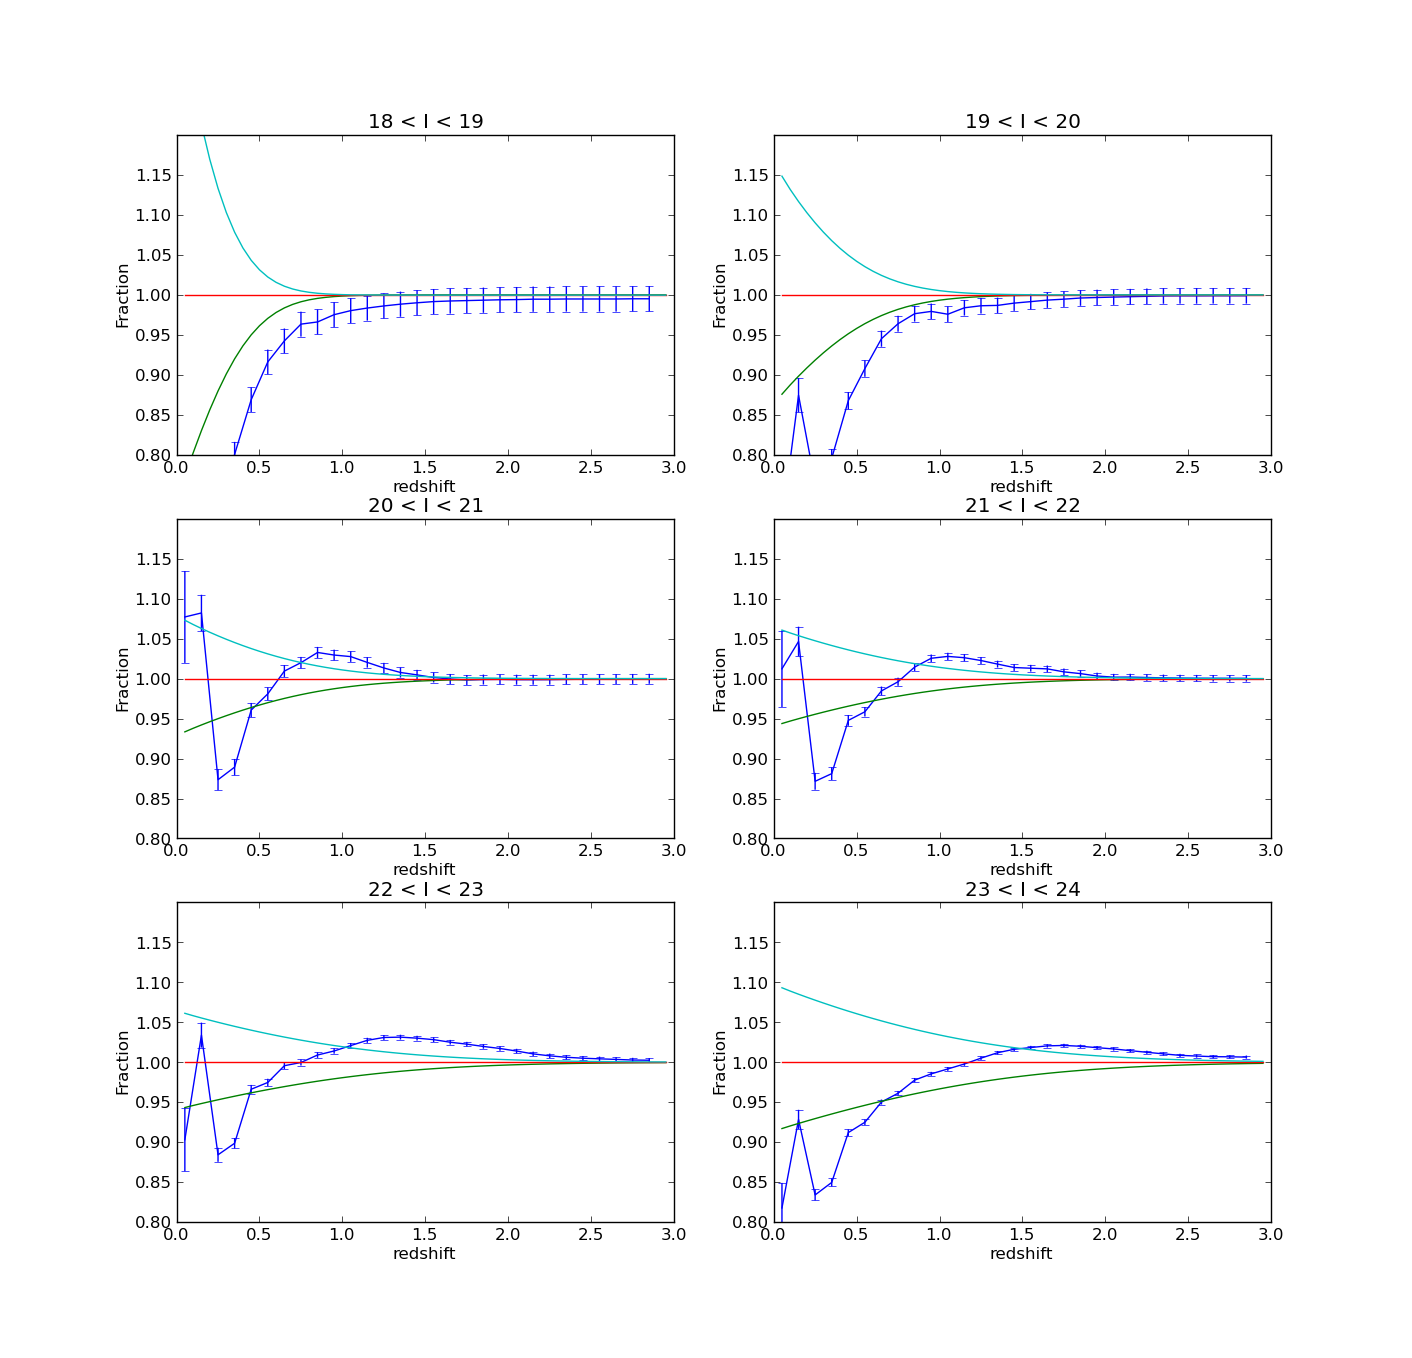
\includegraphics[width=5in]{validation_figures/Nofz_CumulativeFraction_18_24.eps}
\caption{N(z) for 18 to 24 with distribution from \cite{coil}\label{fig:nofz18_24_ratio}}
\end{figure}
\begin{figure}
\centering
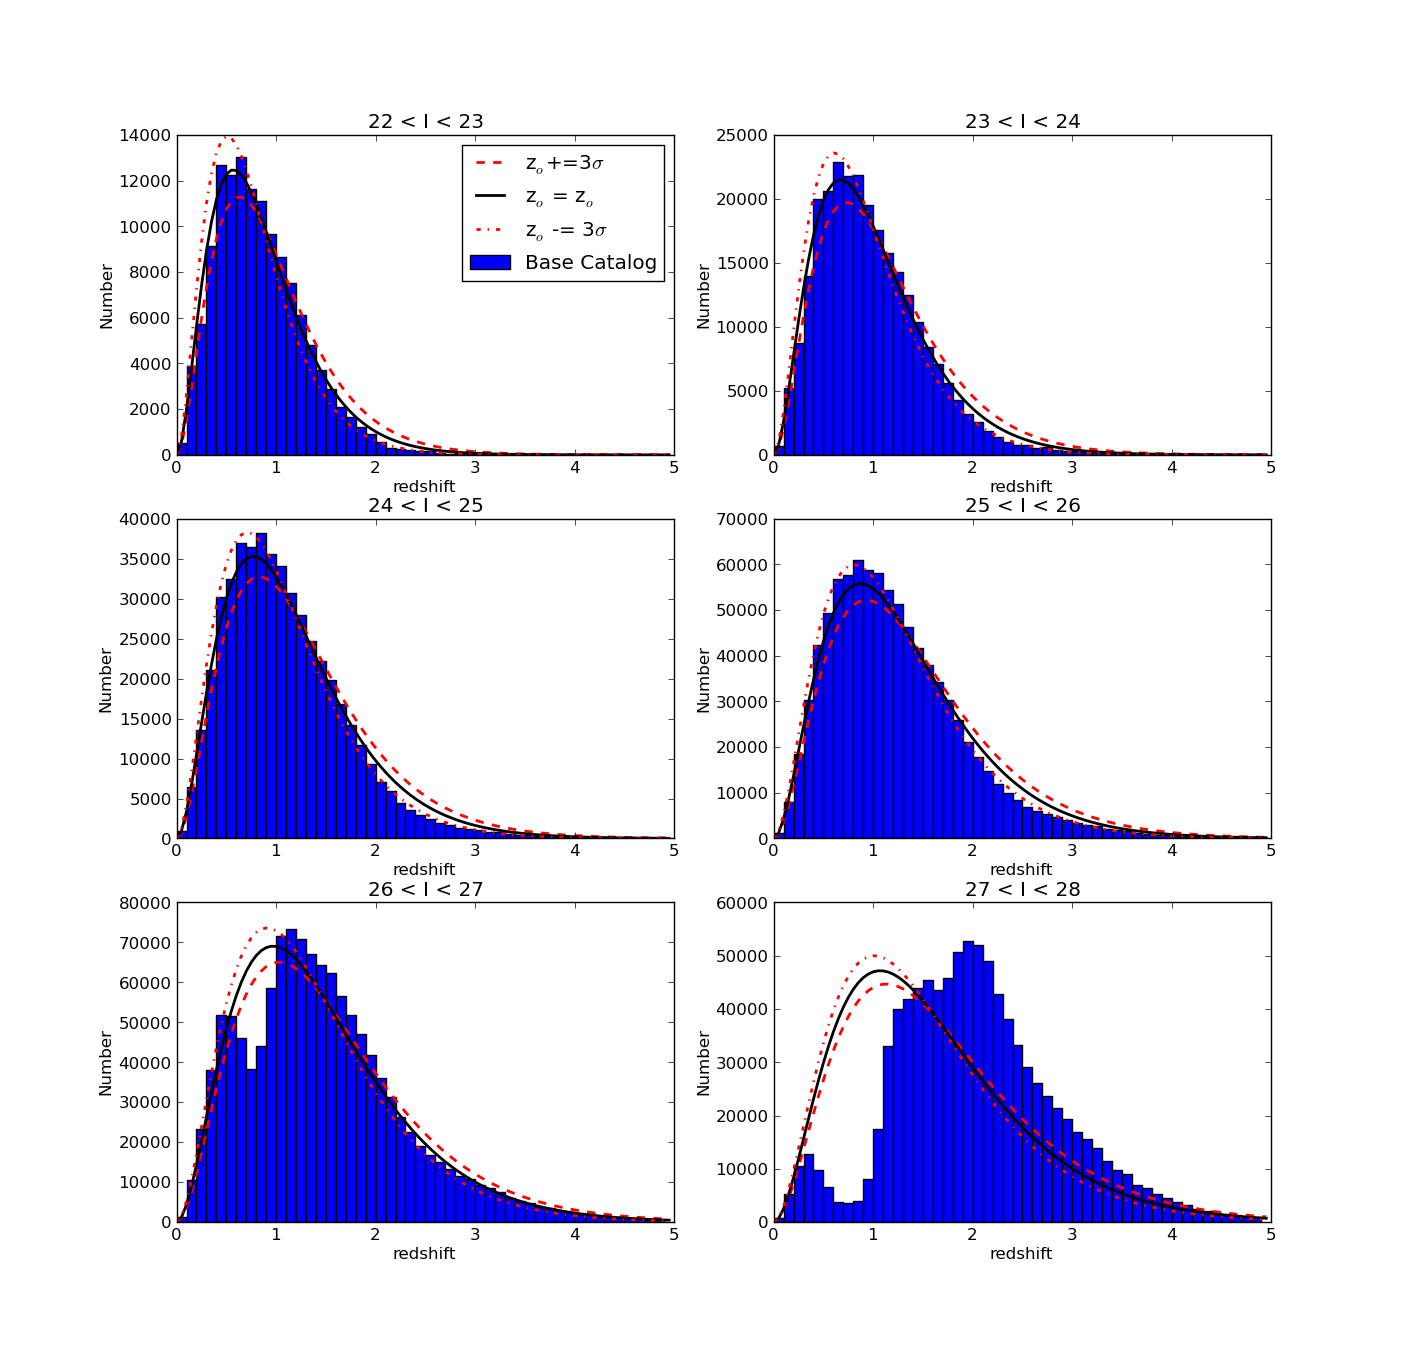
\includegraphics[width=5in]{validation_figures/Nofz_coil_22_28.eps}
\caption{N(z) for 22 to 28 with distribution from \cite{coil}\label{fig:nofz22_28}}
\end{figure}
\begin{figure}
\centering
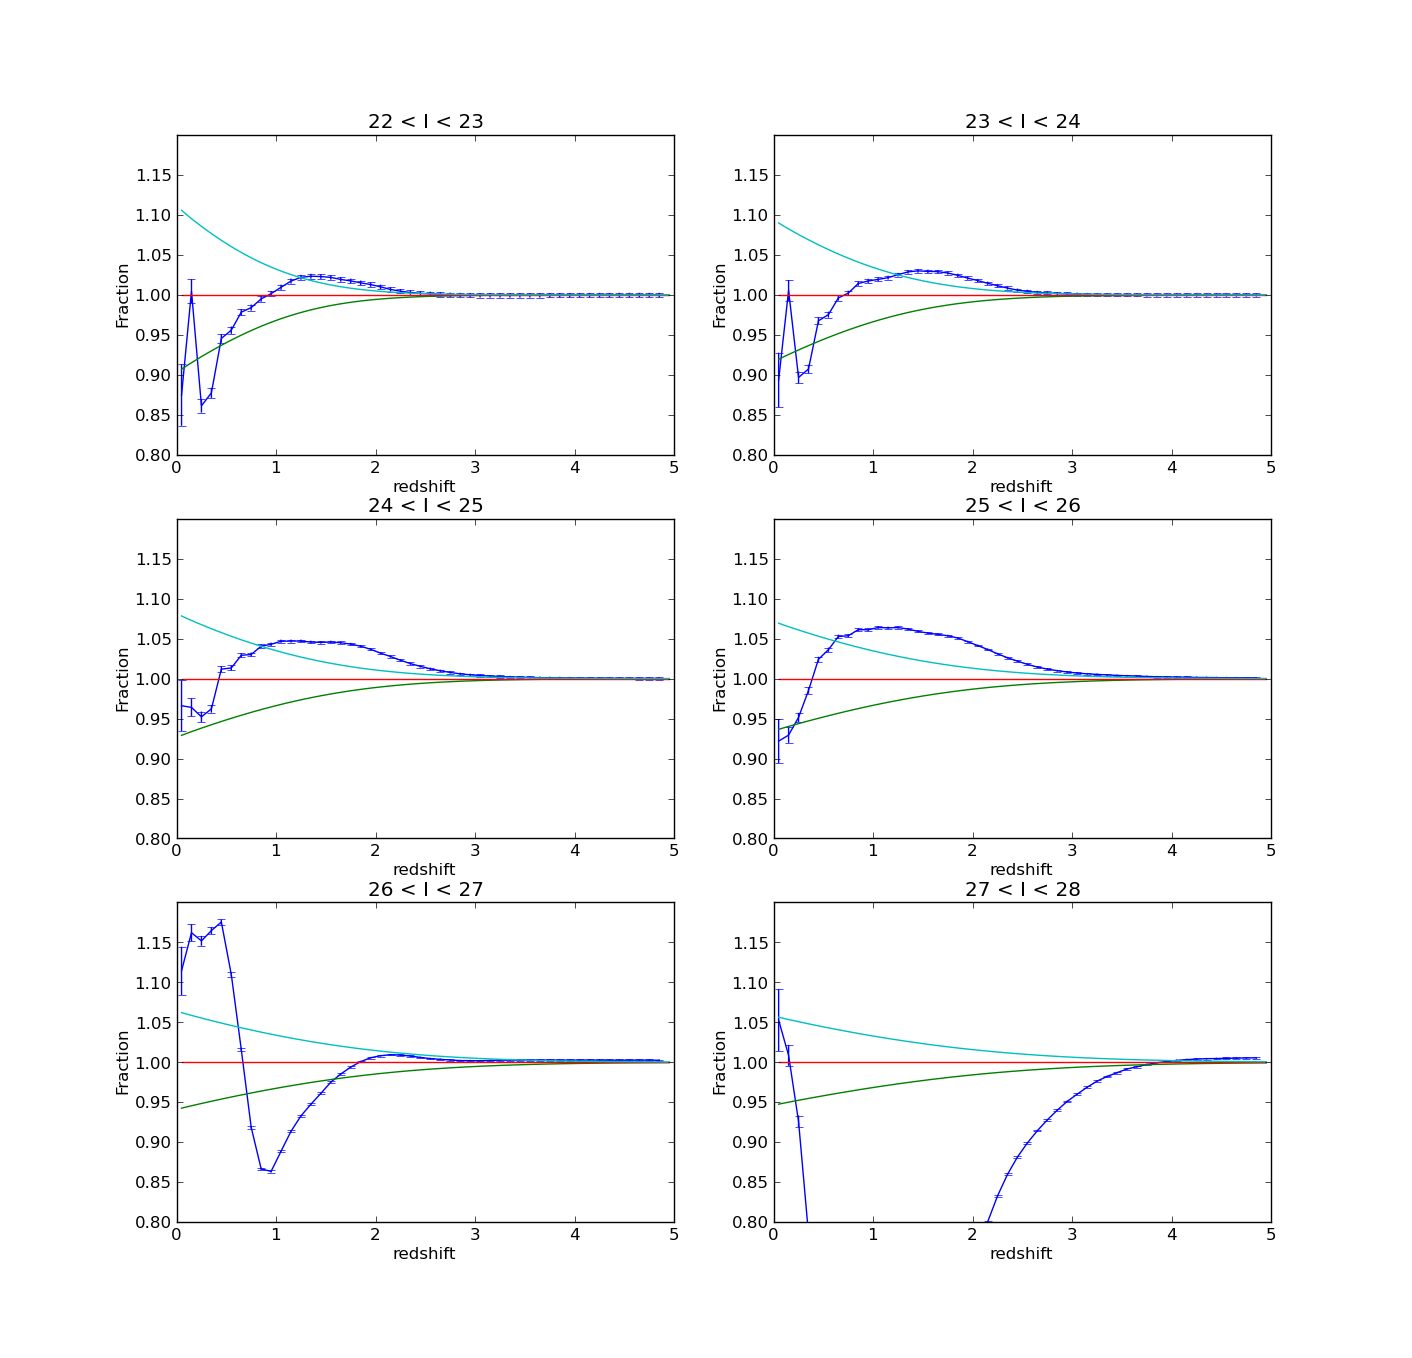
\includegraphics[width=5in]{validation_figures/Nofz_CumulativeFraction_22_28.eps}
\caption{N(z) for 22 to 28 with distribution from \cite{coil}\label{fig:nofz22_28_ratio}}
\end{figure}

\subsection{Requirement 4: For the photometric calibration simulations
the distribution of stellar colors shall encompass the colors of white dwarfs through red giant branch stars.
The median color distributions of stars must trace the observed colar locus for these stars to within 0.02 magnitudes
of the principal color (s,w,x,y) to the designed 5$\sigma$ single epoch limiting magnitude in the r-band.
{\bf update this for the most recent statement in the requirements document}}
For several reasons from calibration through to stellar populations work the Galactic model must have realistic color distributions.
This goes beyond simply spanning the proper color ranges.  The main sequence stellar locus must also agree with the location of the
stellar locus from other projects.  In Figure \ref{fig:starcolorspan} we show that the more trivial requirement that the stellar
colors span the ranges given in the requirements document is met.  Dashed lines in each panel show the requirements.  The measured
color distribution is plotted in the histogram.  The main sequence and red giant branch (RGB) contributions are plotted separately from
the white dwarf population.  Together the two distributions cover the required range.  The y-axis is log scale.

To verify the veracity of the main sequence stellar locus, we use the principal colors of the stellar locus defined by \cite{ivezic04}.
We use stars selected from the same fields as used in the number counts analysis for all fields south of a galactic latitude of -30.
In order to avoid complications associated with the difference between the LSST and SDSS photometric systems, we calculate the un-extincted 
magnitudes in the SDSS bandpasses using the best fit spectrum for each star.  We then calculate
the principal colors for each star using the relations in \cite{ivezic04}, but removing the r-band dependence in $P\prime_{2}$.  Figure
\ref{fig:principalcolors} shows that the principal colors as calculated from the base catalog are in very good agreement with
the location of the stellar locus in the SDSS (zero color).  The base catalog easily meets the requirement of $\pm0.05mag$ deviation
from the stellar locus to single epoch depth in all 4 principal colors.  The scatter and trend with magnitude in the s color is due to 
the sensitivity of u-band on $[$Fe$/$H$]$.  Figure \ref{fig:sfeh} shows this dependence.  The transition from high metalicity disk stars to low 
metalicity halo stars introduces the scatter and slope.

Figure \ref{fig:principalcolorshist} shows that the requirement of mean deviation from the color locus defined by the four principal colors by less than 
0.02 magnitudes is met in all four bands.
\begin{figure}
\centering
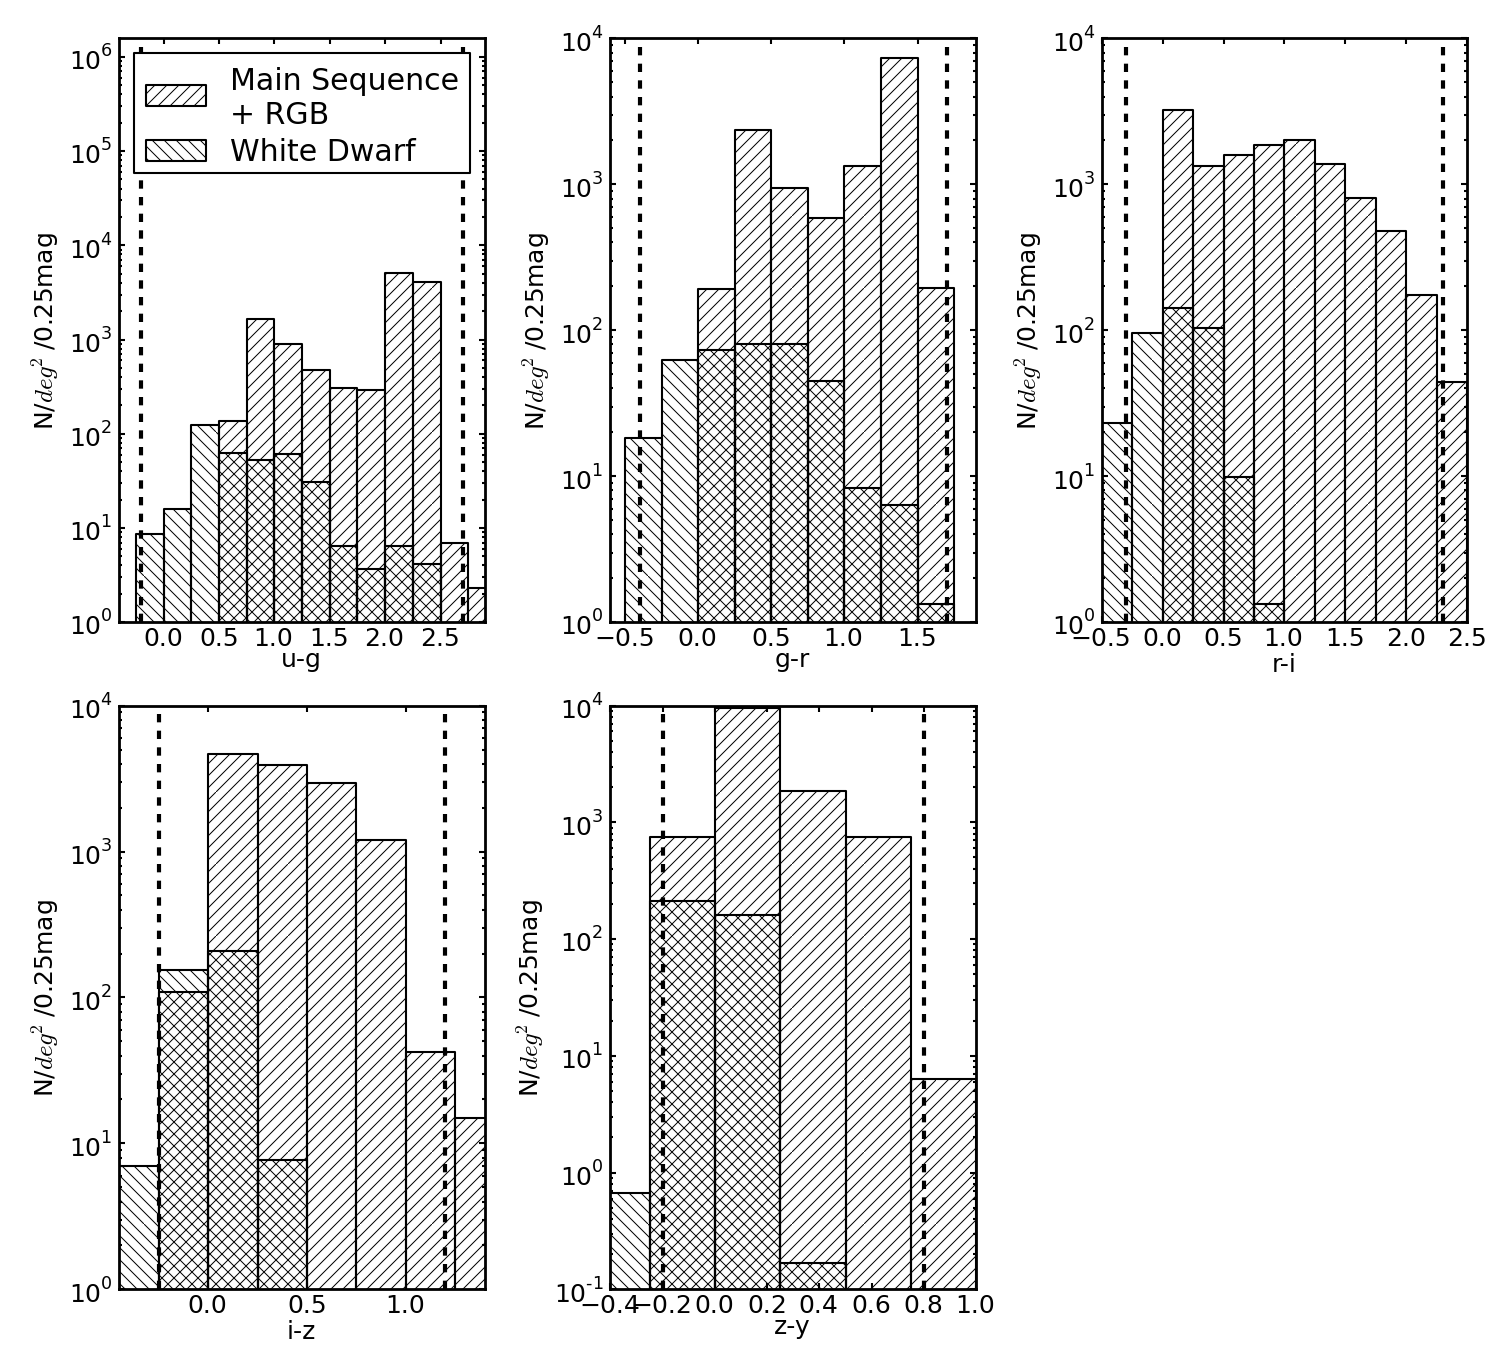
\includegraphics[width=5in]{validation_figures/star_lsst_color_hist.eps}
\caption{Normalized counts of main sequence, red giant branch and white dwarf stars.  Heavy dashed lines show the requirements stated in the requirements document.\label{fig:starcolorspan}}
\end{figure}

\begin{figure}
\centering
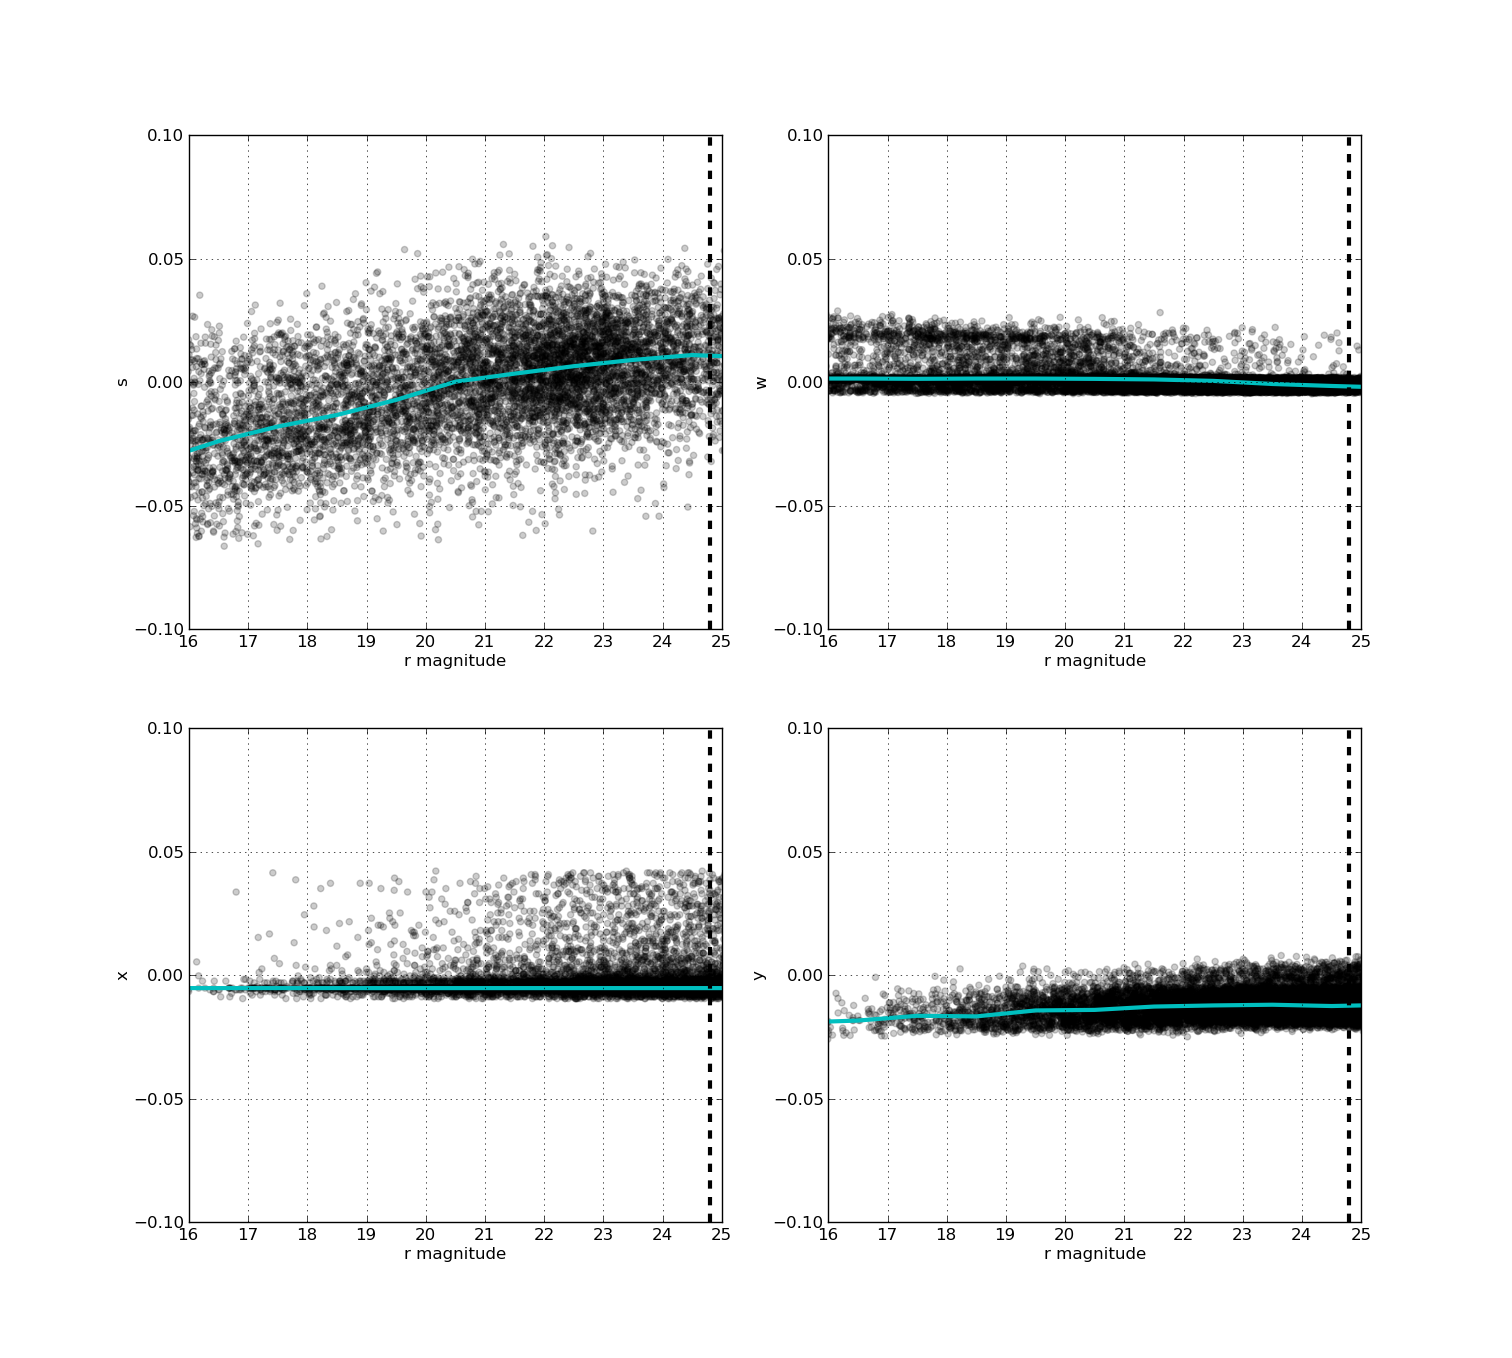
\includegraphics[width=5in]{validation_figures/principal_colors_vr.eps}
\caption{Principal colors for the base catalog compared to the location of the stellar locus in the SDSS.\label{fig:principalcolors}}
\end{figure}

\begin{figure}
\centering
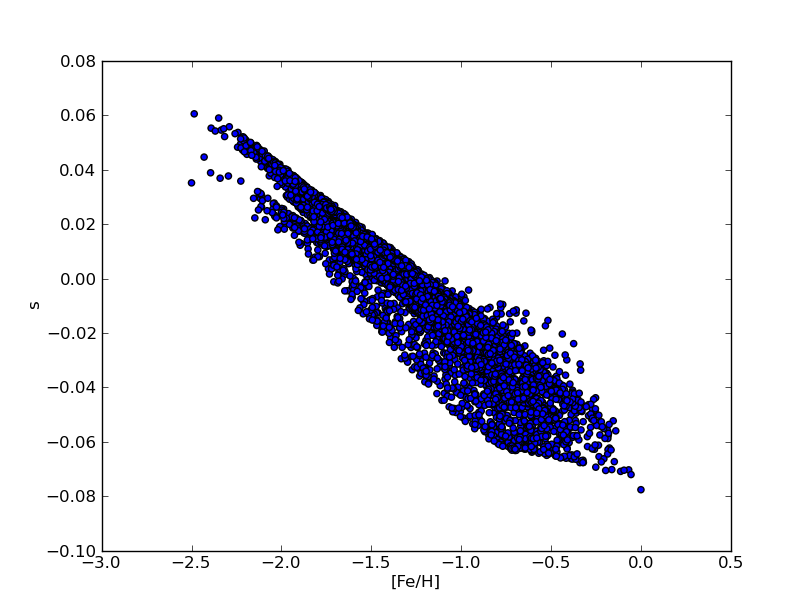
\includegraphics[width=5in]{validation_figures/s_met.eps}
\caption{The principal color 's' as a function of metalicity.\label{fig:sfeh}}
\end{figure}

\begin{figure}
\centering
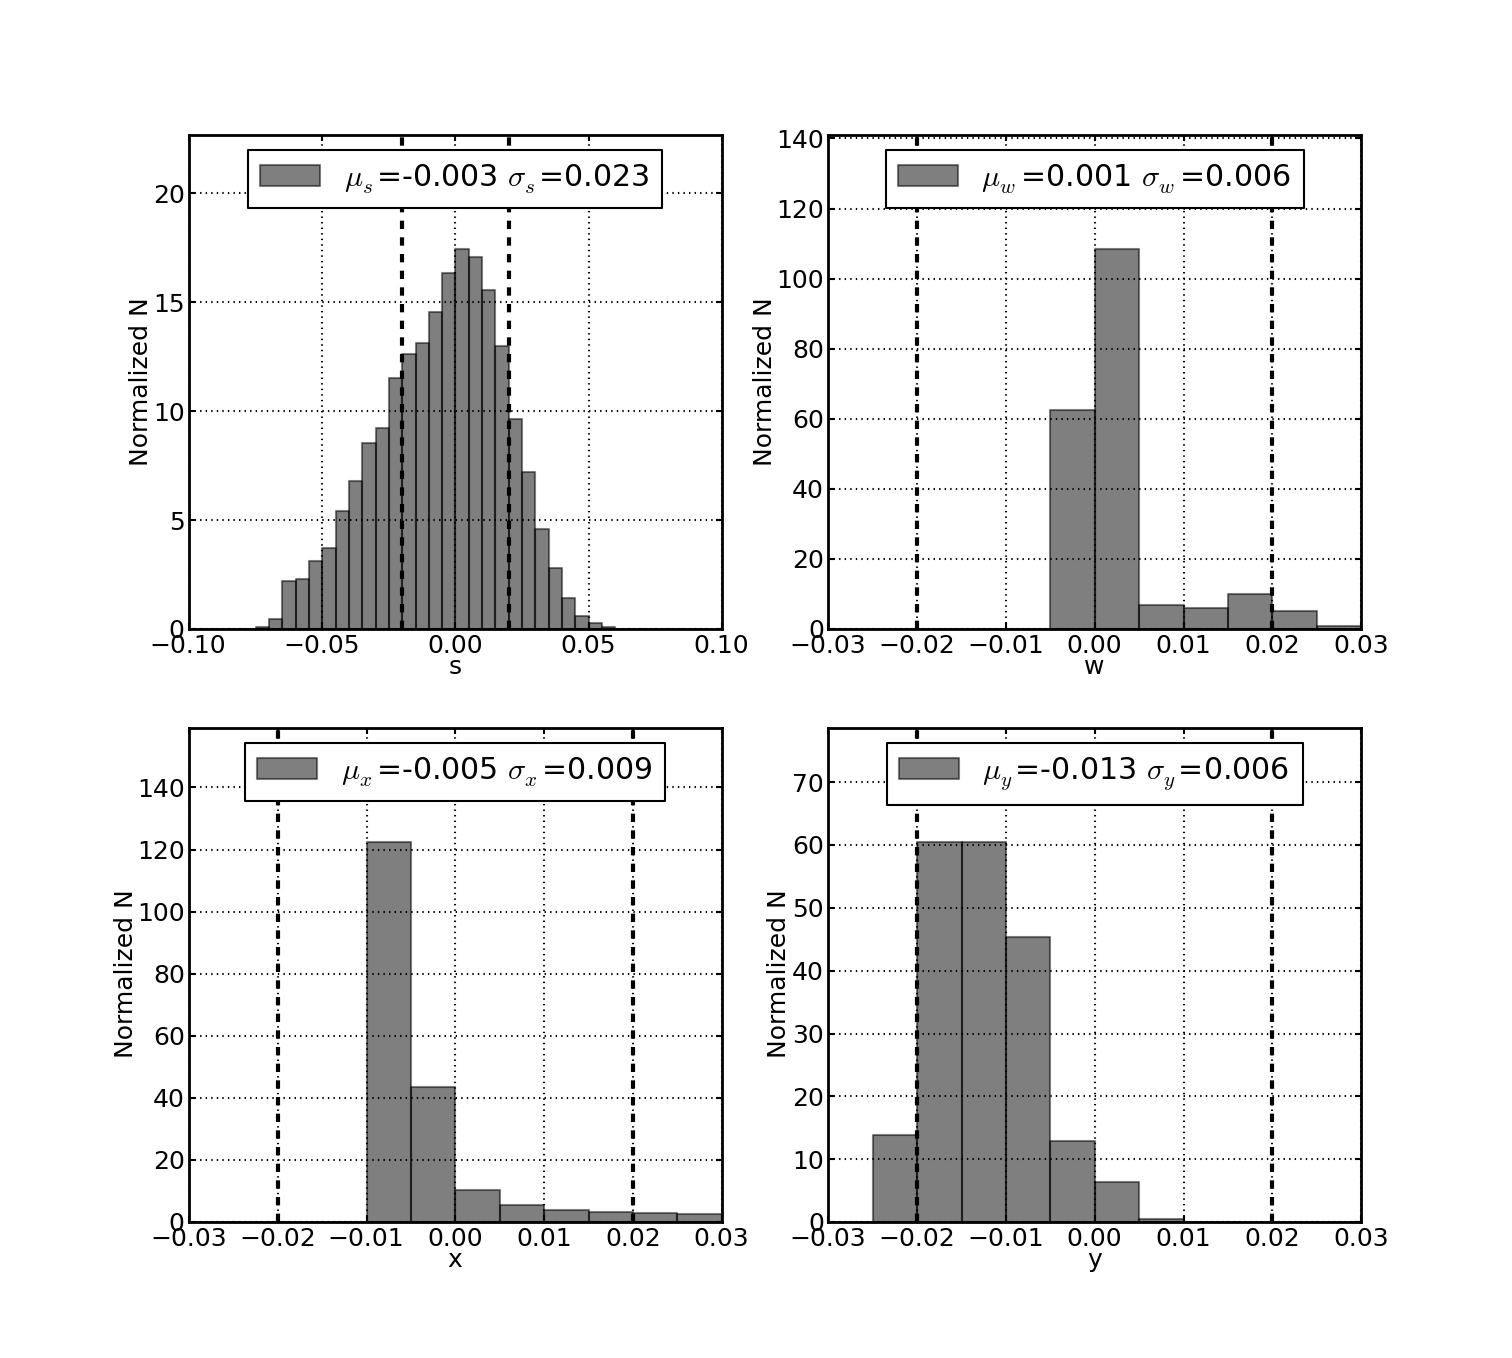
\includegraphics[width=5in]{validation_figures/principal_colors_hist.eps}
\caption{Hisograms of the principal colors of stars in the base catalog to the stretch depth of r < 24.8. The mean and standard deviation for each 
histogram are given in the legend in the upper right.\label{fig:principalcolorshist}}
\end{figure}
\subsection{Requirement 5: All models for the astrometric transforms applied tothe catalogs (including interpolation functions) 
shall have an accuracy better than 1.6 mas}
{\bf XXX Need help from AJC and Yusra on this one.}
\subsection{Requirement 6: The system shall be capable of incorporating new astrophysical catalogs without requiring
a redesign of the class-schema framework}
{\bf XXX Still not sure here.  Do we simply show a snippet of code that describes how one would add a new catalog?}
\end{document}
